\subsection{Experiment Details}
The tests were run on a laptop using a few scripts to automate the testing and formatting of data. Valgrind with the Massif heap profiler was used to obtain data about the size of memory used during testing. This heap profiling was done in a seperate test run to not affect the running times of the main test.
Each test was run with various amounts of operations, all powers of 2: $2^{18}=262144$, $2^{19}=524288$, $2^{20}=1048576$, $2^{21}=2097152$, $2^{22}=4194304$, $2^{23}=8388608$ and $2^{24}=16777216$. The number of operations is given to each test as input parameter $n$.

\subsubsection{Test Types}
Three types of test was done:
\begin{description}
\item[TestInserts] Testing the running time of Insert operations by measuring the time it takes to insert elements $n-1$ to $0$ in that order.
\item[TestDeleteMin] Testing the running time of DeleteMin operations by first inserting elements like in the TestInserts test without measuring the time and then running DeleteMin the same amount of times while measuring time.
\item[TestInterleaved] Testing the running time of interleaved Insert and DeleteMin operations by first inserting elements $n-1$ to $\frac{n-1}{2}$ elements without measuring time, and then interleaved calling DeleteMin and Insert on elements $\frac{n-1}{2}$ to $0$ while measuring time.
\end{description}



\subsection{Expectations}

We expect the Van Emde Boas Trees to perform quite well in terms of speed. Their upper bound on comparisons and general operations of $O(\log (\log U))$, will most likely  make them outperform the more general heaps, especially as data sizes grow.

In terms of memory, we known that the Van Emde Boas Trees will use a large constant amount of memory, though we expect the Van Emde Boas tree with bit magic will use a smaller amount of memory than the other heaps as the universe grows full, due to not actually storing the entire value of the elements.

\subsection{Data}

\subsubsection{Running Times}
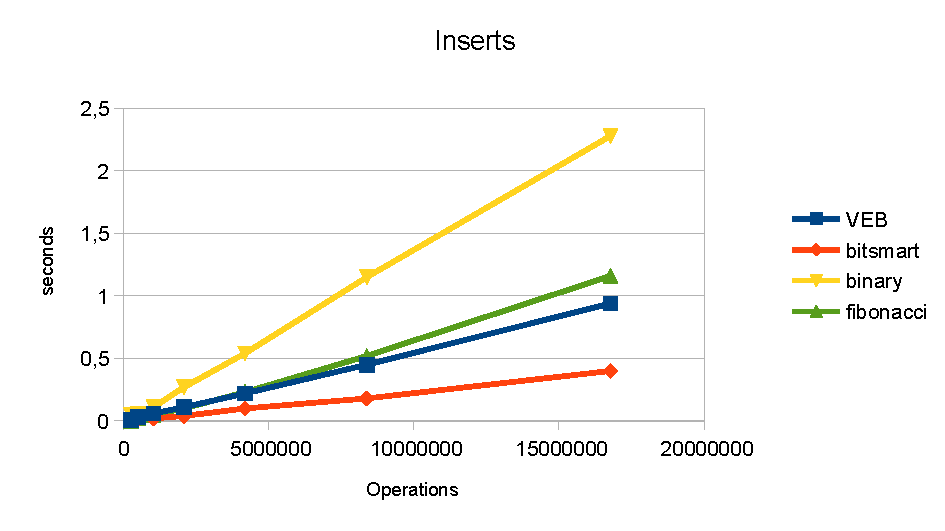
\includegraphics[width=\textwidth]{graphs/Inserts.pdf}
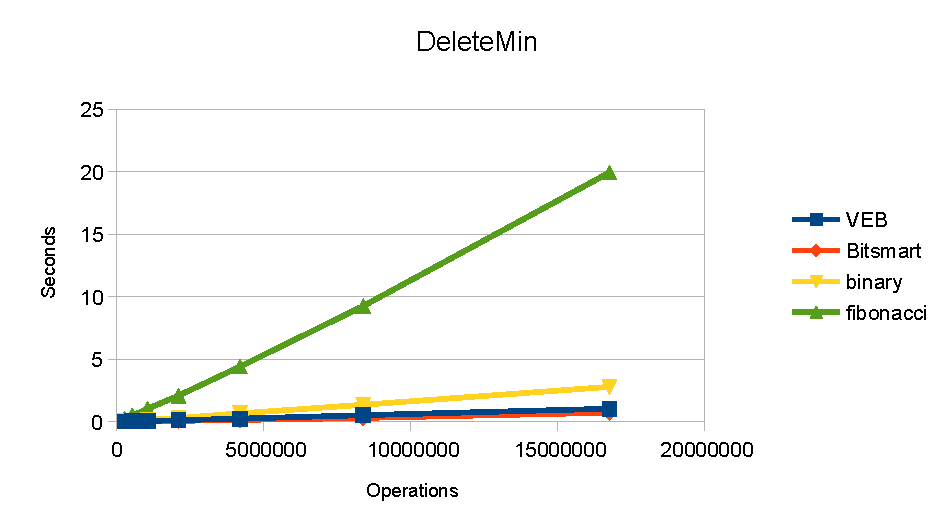
\includegraphics[width=\textwidth]{graphs/DeleteMin.pdf}
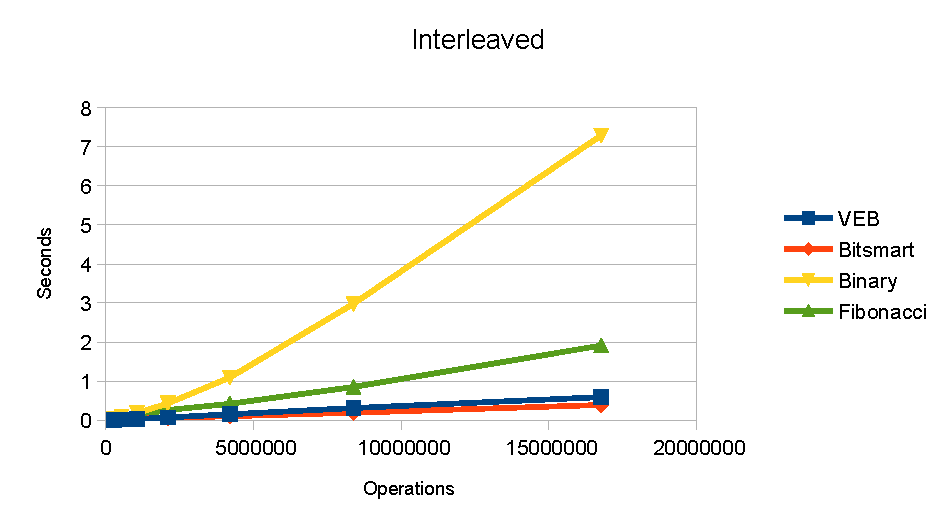
\includegraphics[width=\textwidth]{graphs/Interleaved.pdf}

\subsubsection{Comparisons}
We have been slightly more aggressive in counting comparisons in our van Emde Boas tree implementation, so we might be under counting the comparisons used in the binary and fibonacci heaps compared to the van Emde Boas heaps.
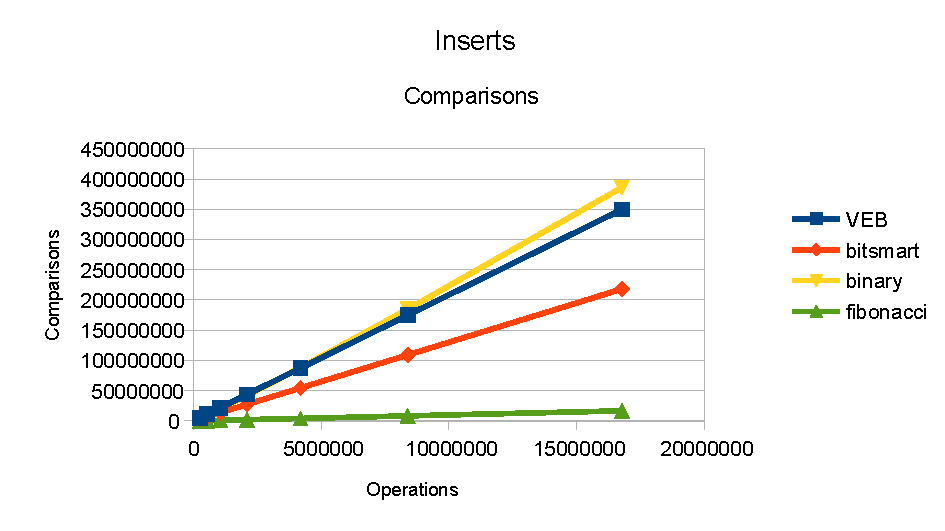
\includegraphics[width=\textwidth]{graphs/Inserts_comparisons.pdf}
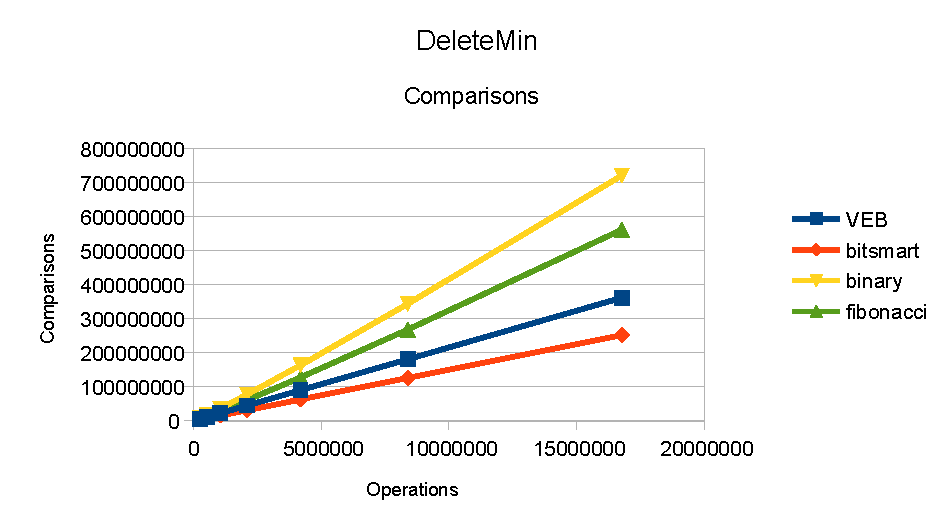
\includegraphics[width=\textwidth]{graphs/DeleteMin_comparisons.pdf}
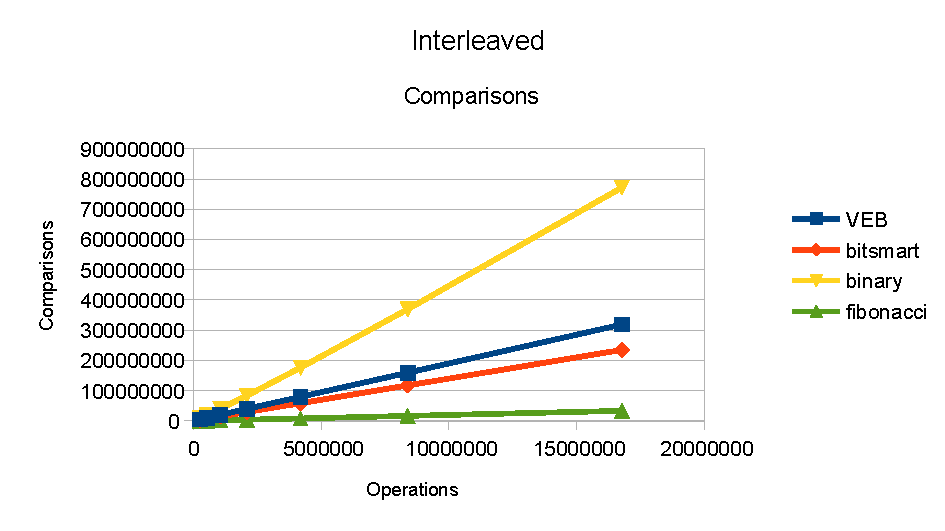
\includegraphics[width=\textwidth]{graphs/Interleaved_comparisons.pdf}

\subsubsection{Memory}
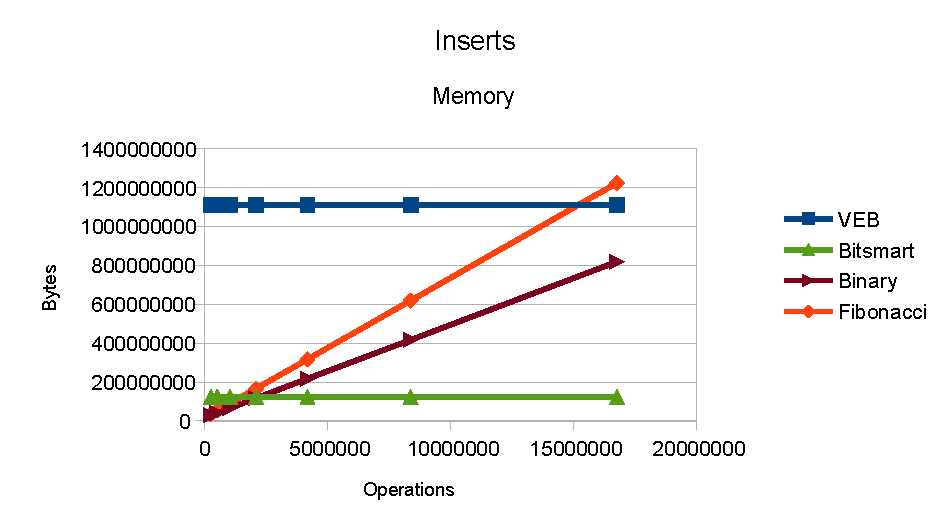
\includegraphics[width=\textwidth]{graphs/Inserts_memory.pdf}
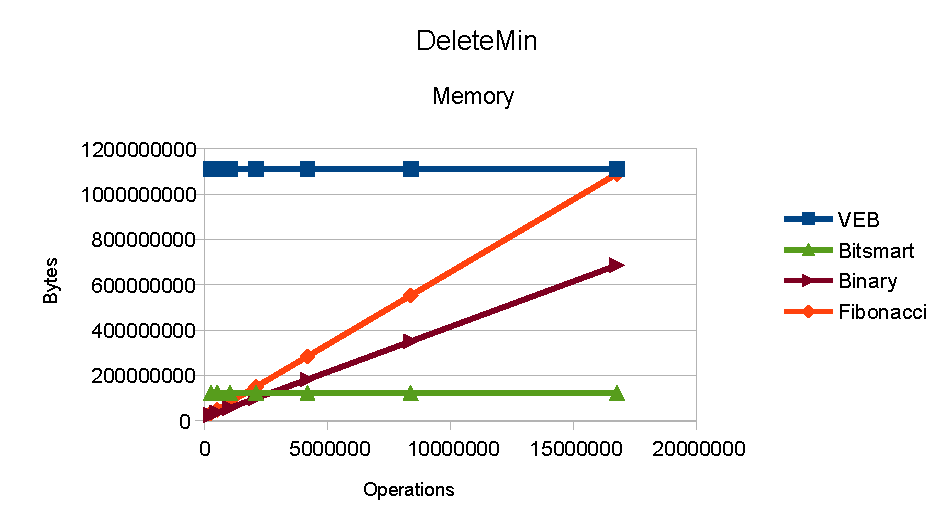
\includegraphics[width=\textwidth]{graphs/DeleteMin_memory.pdf}
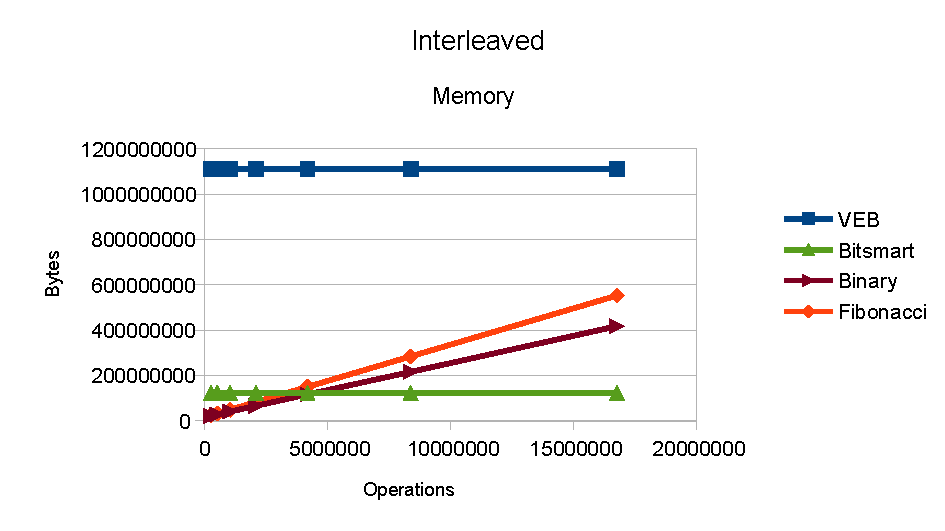
\includegraphics[width=\textwidth]{graphs/Interleaved_memory.pdf}



\subsection{Results}

We see that our experiments behave much as we expected. The Van Emde Boas Tree  based heap are much faster than the ordinary heaps, and using bit magic gives a small, yet significant speed boost. They even outperform Fibonacci Heaps on inserts, which is quite impressive.

In terms of memory we can see that the ordinary Van Emde Boas Tree uses a huge amount of memory, only being surpassed by the Fibonacci Heap at a full universe. The bit magic Van Emde boas tree on the other hand uses a quite acceptable amount of memory, being roughly equal with the other heaps at about 2 million elements.